\documentclass[10pt,a4paper,twocolumn]{article}
\usepackage[a4paper,margin=17mm,columnsep=6mm]{geometry}
\usepackage[T1]{fontenc}
\usepackage{newtxtext,newtxmath}
\usepackage{microtype}
\usepackage{amsmath}
\usepackage{booktabs}
\usepackage{graphicx}
\usepackage{xcolor}
\usepackage[font=small,labelfont=bf,skip=4pt]{caption}
\usepackage{enumitem}
\usepackage[hidelinks]{hyperref}
\usepackage{tabularx}
\usepackage{array}
\setlist{nosep,leftmargin=*}
\graphicspath{{fig/}}
\newcommand{\Tab}[1]{\input{tab/tab_#1.tex}}
\newcommand{\NBflapMod}{1.11}
\newcommand{\NBlagBeam}{0.76}
\newcommand{\NBlagMod}{0.67}
\newcommand{\NBlagScale}{0.19}
\newcommand{\NBtorsMod}{3.80}
\newcommand{\NDbAll}{2.1}
\newcommand{\NDbLonPk}{$-$7.1}
\newcommand{\NDbLonPkT}{$-$6.9}
\newcommand{\NDbOn}{0.045}
\newcommand{\NDbOnDeg}{2.6}
\newcommand{\NDbPedPk}{14}
\newcommand{\NDbPedPkT}{13}
\newcommand{\NDbPedR}{4.4}
\newcommand{\NDerIn}{17}
\newcommand{\NDerN}{36}
\newcommand{\NDhoverTq}{7.87}
\newcommand{\NDhoverTqTest}{8.92}
\newcommand{\NDhoverTqTestV}{4}
\newcommand{\NDlatMax}{0.2}
\newcommand{\NDlatMin}{$-$1.4}
\newcommand{\NDlonMax}{1.3}
\newcommand{\NDlonMaxHi}{0.6}
\newcommand{\NDlonMin}{0.2}
\newcommand{\NDphi}{$-$1.7}
\newcommand{\NDpitchMax}{1.3}
\newcommand{\NDrollMax}{$-$1.3}
\newcommand{\NDrollMin}{$-$3.3}
\newcommand{\NDtheta}{$-$1.6}
\newcommand{\NDthzMax}{1.1}
\newcommand{\NDthzMin}{0.5}
\newcommand{\NDtqLow}{4}
\newcommand{\NDtqMax}{2}
\newcommand{\NDtqMin}{$-$9}
\newcommand{\NDtrHi}{0.5}
\newcommand{\NDtrMax}{2.3}
\newcommand{\NDtrMaxV}{30}
\newcommand{\NEazRms}{0.49}
\newcommand{\NEnrMaxM}{0.78}
\newcommand{\NEnrMaxT}{1.03}
\newcommand{\NEnrMinM}{$-$1.19}
\newcommand{\NEnrMinT}{$-$1.32}
\newcommand{\NEnrPct}{0.39}
\newcommand{\NEnrRms}{0.17}
\newcommand{\NEtqMaxM}{1.9}
\newcommand{\NEtqMaxT}{1.3}
\newcommand{\NEtqMinM}{$-$1.4}
\newcommand{\NEtqMinT}{$-$1.9}
\newcommand{\NFgainLow}{$-$33.3}
\newcommand{\NFgainLowT}{$-$33.9}
\newcommand{\NFinDthHi}{0.07}
\newcommand{\NFinDthHover}{0.08}
\newcommand{\NFinDthMax}{0.2}
\newcommand{\NFinDthMaxV}{30}
\newcommand{\NFinHiPct}{2}
\newcommand{\NFinHoverLb}{4}
\newcommand{\NFinHoverPct}{1.3}
\newcommand{\NFinPeakLb}{10}
\newcommand{\NFinPeakPct}{4}
\newcommand{\NFinPeakV}{30}
\newcommand{\NFmagMax}{1.8}
\newcommand{\NFmagRms}{1.0}
\newcommand{\NFphHi}{25}
\newcommand{\NFphMax}{14}
\newcommand{\NFphRms}{7}
\newcommand{\NHcpMax}{11}
\newcommand{\NHcpMin}{3}
\newcommand{\NHfmMod}{0.73}
\newcommand{\NHfmTest}{0.66}
\newcommand{\NHthMax}{3.1}
\newcommand{\NHthMin}{2.6}
\newcommand{\NHtorsMod}{$-$333}
\newcommand{\NHtorsTest}{$-$480}
\newcommand{\NLagCt}{0.070}
\newcommand{\NLagCtHi}{0.098}
\newcommand{\NLagCtLo}{0.031}
\newcommand{\NLagMod}{$-$1.02}
\newcommand{\NLagModHi}{$-$1.30}
\newcommand{\NLagModLo}{$-$0.68}
\newcommand{\NLagNu}{0.66}
\newcommand{\NLagTest}{$-$0.97}
\newcommand{\NLagTestHi}{$-$1.60}
\newcommand{\NLagTestLo}{$-$0.56}
\newcommand{\NMcoll}{1.0}
\newcommand{\NMdrPct}{6}
\newcommand{\NMdrW}{2.75}
\newcommand{\NMdrZeta}{0.20}
\newcommand{\NMlat}{0.9}
\newcommand{\NMlon}{1.2}
\newcommand{\NMlonHi}{0.4}
\newcommand{\NMpTwo}{0.46}
\newcommand{\NMphW}{0.28}
\newcommand{\NMphZeta}{$-$0.13}
\newcommand{\NMpitch}{1.2}
\newcommand{\NMpowMin}{307}
\newcommand{\NMpowMinV}{55}
\newcommand{\NMrpW}{8.95}
\newcommand{\NMrpZeta}{1.00}
\newcommand{\NSsPitch}{2.0}
\newcommand{\NSsPitchDlr}{2.7}
\newcommand{\NSsRoll}{1.9}
\newcommand{\NSsRollDlr}{2.2}
\newcommand{\NTrBaHi}{1.1}
\newcommand{\NTrBaHover}{+0.4}
\newcommand{\NTrBaHoverPow}{32}
\newcommand{\NTrBaTransMax}{3.6}
\newcommand{\NTrBaTransMin}{3.0}
\newcommand{\NTrBeHi}{0.5}
\newcommand{\NTrBeHover}{$-$1.4}
\newcommand{\NTrBeHoverDeg}{9.4}
\newcommand{\NTrBeHoverPow}{34}
\newcommand{\NTrBeTransMax}{2.3}
\newcommand{\NTrBeTransMin}{1.4}
\newcommand{\NTrHoverTest}{10.8}
\newcommand{\NdLcol}{$-$0.016}
\newcommand{\NdLcolDlr}{0.032}
\newcommand{\NdLcolHi}{0.058}
\newcommand{\NdLcolLo}{0.004}
\newcommand{\NdLlat}{0.200}
\newcommand{\NdLlatDlr}{0.185}
\newcommand{\NdLlatHi}{0.185}
\newcommand{\NdLlatLo}{0.053}
\newcommand{\NdLlon}{$-$0.072}
\newcommand{\NdLlonDlr}{0.024}
\newcommand{\NdLlonHi}{0.073}
\newcommand{\NdLlonLo}{$-$0.005}
\newcommand{\NdLp}{$-$10.585}
\newcommand{\NdLpDlr}{$-$8.501}
\newcommand{\NdLpHi}{$-$1.995}
\newcommand{\NdLpLo}{$-$8.779}
\newcommand{\NdLv}{$-$0.261}
\newcommand{\NdLvDlr}{$-$0.271}
\newcommand{\NdLvHi}{$-$0.038}
\newcommand{\NdLvLo}{$-$0.271}
\newcommand{\NdMcol}{0.090}
\newcommand{\NdMcolDlr}{0.057}
\newcommand{\NdMcolHi}{0.073}
\newcommand{\NdMcolLo}{0.032}
\newcommand{\NdMlon}{0.138}
\newcommand{\NdMlonDlr}{0.093}
\newcommand{\NdMlonHi}{0.098}
\newcommand{\NdMlonLo}{0.050}
\newcommand{\NdMp}{$-$1.201}
\newcommand{\NdMpDlr}{$-$0.419}
\newcommand{\NdMpHi}{$-$0.419}
\newcommand{\NdMpLo}{$-$1.414}
\newcommand{\NdMq}{$-$6.754}
\newcommand{\NdMqDlr}{$-$3.496}
\newcommand{\NdMqHi}{$-$1.441}
\newcommand{\NdMqLo}{$-$4.493}
\newcommand{\NdMw}{0.084}
\newcommand{\NdMwDlr}{0.053}
\newcommand{\NdMwHi}{0.356}
\newcommand{\NdMwLo}{0.019}
\newcommand{\NdNp}{0.031}
\newcommand{\NdNpDlr}{$-$1.057}
\newcommand{\NdNpHi}{$-$0.466}
\newcommand{\NdNpLo}{$-$1.958}
\newcommand{\NdNped}{0.081}
\newcommand{\NdNpedDlr}{0.049}
\newcommand{\NdNpedHi}{0.484}
\newcommand{\NdNpedLo}{0.043}
\newcommand{\NdNr}{$-$1.094}
\newcommand{\NdNrDlr}{$-$0.858}
\newcommand{\NdNrHi}{$-$0.699}
\newcommand{\NdNrLo}{$-$1.116}
\newcommand{\NdNv}{0.178}
\newcommand{\NdNvDlr}{0.117}
\newcommand{\NdNvHi}{0.117}
\newcommand{\NdNvLo}{0.051}
\newcommand{\NdZcol}{$-$0.267}
\newcommand{\NdZcolDlr}{$-$0.349}
\newcommand{\NdZcolHi}{$-$0.242}
\newcommand{\NdZcolLo}{$-$0.388}
\newcommand{\NdZw}{$-$0.757}
\newcommand{\NdZwDlr}{$-$0.998}
\newcommand{\NdZwHi}{$-$0.791}
\newcommand{\NdZwLo}{$-$1.187}
\newcommand{\NnFcs}{427}
\newcommand{\NnFunc}{985}

\newcommand{\ok}{\textcolor{green!45!black}{\ensuremath{\checkmark}}}
\newcommand{\nok}{\textcolor{red!70!black}{\ensuremath{\times}}}
\newcommand{\pok}{\textcolor{orange!85!black}{\ensuremath{\sim}}}
\renewcommand{\arraystretch}{1.08}
\setlength{\tabcolsep}{4pt}
\raggedbottom
\renewcommand{\topfraction}{0.92}\renewcommand{\dbltopfraction}{0.92}\renewcommand{\bottomfraction}{0.6}
\renewcommand{\textfraction}{0.06}\renewcommand{\floatpagefraction}{0.85}\renewcommand{\dblfloatpagefraction}{0.85}
\setcounter{topnumber}{3}\setcounter{dbltopnumber}{3}\setcounter{totalnumber}{5}
\makeatletter\setlength{\@fptop}{0pt}\setlength{\@dblfptop}{0pt}\makeatother
\begin{document}

\twocolumn[
\begin{@twocolumnfalse}
\begin{center}
{\LARGE\bfseries Flight Dynamics of the MBB Bo 105 in JSBSim\par}
\vspace{6pt}
{\large\bfseries An elastic-blade hingeless rotor model, checked against DLR and MBB flight tests and NASA's full-scale rotor tests\par}
\vspace{10pt}
{\large Technical report \quad\textbullet\quad October 2026\par}
\vspace{10pt}
\end{center}
\begin{abstract}
\noindent
A flight-dynamics model of the MBB Bo 105 for the FlightGear simulator has been written in JSBSim, replacing the
parametric YASim model the aircraft used before. The Bo 105's hingeless, soft in-plane rotor is what sets it apart, and the
model is built around it: the four blades are simulated individually as elastic beams cantilevered from the hub with
2.5$^\circ$ of precone, each with its first flap and lag bending modes, computed from the blade's mass and stiffness
distribution, and a quasi-static first torsion mode; eight segments per blade use the NACA 23012 tables of Boeing Vertol's
C-81 analysis at their own angle of attack and Mach number, under a Peters--He finite-state dynamic wake. The hub moments come
from the blades' root bending, the rotor speed and the four lag accelerations are solved together, and a ring-vortex wake
carries the rotor's downwash to the fuselage, stabiliser, end plates and tail rotor. A blade-element teetering tail rotor and two Allison
250-C20B engines with their governors complete it. The whole model, \NnFunc{} aerodynamic functions and \NnFcs{} control-system components, is generated by a
script from transcribed data and runs in plain JSBSim at 960\,Hz without scripting. It was flown offline through a scripted
programme. Level-flight trims agree with MBB's flight test within \NMcoll$^\circ$ of collective, \NMlon$^\circ$ of longitudinal and
\NMlat$^\circ$ of lateral cyclic and \NMpitch$^\circ$ of pitch attitude up to 118\,kt, and with the DLR Bo 105-S123 with the collective
\NDthzMin--\NDthzMax$^\circ$ higher and the main rotor torque within \NDtqMin{} to $+$\NDtqMax\,\%. The blades' first flap, lag and torsion frequencies are
\NBflapMod, \NBlagMod{} and \NBtorsMod{} per revolution against 1.12, 0.66 and 3.79 from NASA's analysis, and the lag damping follows the
full-scale rotor's measured decay (\NLagMod{} against \NLagTest\,s$^{-1}$ at $C_T/\sigma=\NLagCt$). At 80\,kt the roll response to lateral
cyclic is within \NFmagRms\,dB (rms) of DLR's identified transfer function from 1 to 12\,rad/s, including the lag/air resonance near 15\,rad/s,
and the rate responses to the four AGARD verification doublets have a mean on-axis rms error of \NDbOnDeg\,deg/s. Deficiencies are
quantified: the isolated rotor in hover needs \NHcpMin--\NHcpMax\,\% less power than the full-scale test at the same thrust and
\NHthMin--\NHthMax$^\circ$ less collective, the tail rotor's pitch is \NTrBeTransMin--\NTrBeTransMax$^\circ$ above DLR's through
the transition from 20 to 40\,kt and \NTrBeHover$^\circ$ from it in the hover, several cross-coupling derivatives at 80\,kt lie outside the spread of six identifications from the same flights, the pitch and roll
damping derivatives are larger than any of them, and in the longitudinal and collective doublets the free model drifts away from the
aircraft after about ten seconds.
\end{abstract}
\vspace{6pt}
\end{@twocolumnfalse}
]

% =====================================================================================================================
\section{Introduction}
The Bo 105 distributed for FlightGear flies on YASim, whose helicopter model builds the rotor from a short list of geometric
parameters and tuning factors. For most helicopters that is a reasonable compromise; for the Bo 105 it misses what made
the aircraft famous. Its titanium hub carries the blades without flapping or lead-lag hinges: the blades bend instead,
their first flap frequency 1.12 times the rotor speed and their first lag frequency 0.66~\cite{pt}. The flap frequency gives a
hub moment three to four times that of an articulated rotor of the same size, hence the quick, crisp control response and
the aerobatic reputation; the low lag frequency puts a regressing lag mode near 15\,rad/s, where it couples with the body's
roll (air resonance) and has to be damped by the blades' own aerodynamics and structure, since there are no lag dampers.

The data to build a physical model exist in public. Boeing Vertol validated its C-81 rotorcraft analysis against MBB's
flight tests of the Bo 105 in 1975 and published the complete input deck, including the blade's mass and stiffness
distribution~\cite{tr}; it is the Bo 105's equivalent of the UH-60's GenHel documentation. The DLR's research Bo 105, S123,
was the subject of a coordinated system identification by six organisations under AGARD~\cite{ar,kal}. NASA tested the
full-scale rotor in hover and in the 40$\times$80\,ft wind tunnel~\cite{pw,wp,pt,pm}, and the DLR documented its engine and
governor model~\cite{hg}.

This report describes a JSBSim~\cite{jsbsim} model built on that material, after a UH-60A model built the same way, and how well it
reproduces the tests. All of the flight model, including the blades' integration, the wake, the engines and the governors, is JSBSim
XML; the FlightGear side only animates and instruments it. All result tables, figures and the numbers quoted from them are
written by the evaluation scripts.

% =====================================================================================================================
\section{Reference data}\label{sec:ref}
\begin{table}[t]
\centering\small
\caption{Sources and what they contribute.}\label{tab:sources}
\begin{tabularx}{\columnwidth}{@{}>{\raggedright\arraybackslash}p{2.55cm}X@{}}
\toprule
Source & Content used \\
\midrule
USAAMRDL TR 75-50~\cite{tr} & C-81 input deck: geometry, rigging, NACA 23012 tables, blade mass and stiffness (Y-71 beam model), fuselage wind tunnel data; MBB's V-4 trim flights (fig.~16) \\
NASA TM-103867~\cite{pt} & blade frequencies tuned to MBB's measurements, section axes, control system stiffness \\
NASA TM-85892, TM-85990~\cite{pw,wp} & full-scale rotor in hover: thrust, power, lag damping against thrust \\
NASA TM-110356~\cite{pm} & full-scale rotor in the wind tunnel; hub drag tare \\
NASA CR-3144~\cite{hf} & geometry, loadings, stations \\
AGARD AR-280~\cite{ar} & DLR Bo 105-S123: loading and inertias; derivatives and modes at 80\,kt from six identifications; verification doublets \\
15th ERF, paper 66~\cite{kal} & identified roll transfer function at 80\,kt (4th/7th order, with the lag mode) \\
23rd ERF, paper 91~\cite{hg} & 250-C20B engine and governor structure; collective 3-2-1-1 in hover with rotor speed and torque \\
Padfield~\cite{pad}, via~\cite{metu} & DLR S123 trims against airspeed (figs.~4.6, 4.10, 4.11) \\
EASA TCDS R.011~\cite{ea} & engine ratings, speeds and limits \\
Flight manual CB-5/CBS-5~\cite{fm} & stations, loading, cockpit, instrument markings, warning lights \\
METU thesis~\cite{metu} & Peters--He finite-state wake equations \\
NASA TN D-234, NACA TR 1319~\cite{heyson,hk} & ground effect in forward flight; ring-vortex wake \\
\bottomrule
\end{tabularx}
\end{table}

Table~\ref{tab:sources} lists the sources; most are scans, and every curve used was digitised from them. A few points of
data reduction matter for the comparisons.
\emph{(i)} The DLR trims are those Padfield plots against his Helisim model; their weight, 2200\,kg, is given there, the
atmosphere is not, and sea level standard is assumed. The pitch harmonics are in Helisim's convention, the collective at the
shaft.
\emph{(ii)} The MBB trims are those of the V-4 prototype's flight 108 as TR-75-50 plots them against C-81: 4500\,lb, 5000\,ft
density altitude, the CG 3.1\,in forward of the rotor reference axis; collective at 0.7\,$R$ and cyclic as swashplate angles.
\emph{(iii)} The six identifications of AR-280 used the same flight data and differ widely: the roll damping $L_p$ ranges from
$-2.0$ to $-8.8$\,s$^{-1}$; their structures differ (equivalent time delays, terms eliminated). The comparison here asks whether the model
lies within that spread. Two printed values ($N_{\delta_r}$ of Glasgow and NAE) are ten times the
others' and probably misprinted.
\emph{(iv)} The verification doublets of AR-280 (figs.~6.2.17 and 6.2.20) were digitised on the figures' common time axis; each of the
four runs is replayed with the recorded increments of all four controls.
\emph{(v)} NASA's rotor tests ran on the Rotor Test Apparatus in the test section of the 40$\times$80\,ft tunnel, the shaft tilted 10$^\circ$
forward, the first harmonic flapping nulled with cyclic.

% =====================================================================================================================
\section{The model}\label{sec:model}
\subsection{Implementation}
A Python script writes the model from the transcribed tables (Table~\ref{tab:model}). JSBSim evaluates aerodynamic functions on
demand, so the function graph must be free of cycles; every quantity that depends on its own past, the blades' modal
coordinates and their rates, the wake states, the rotor speed, the tail rotor's teeter and inflow and the engines' states, therefore lives in
flight-control-system channels, which JSBSim runs once per frame in a fixed order and which can write properties back. These channels
integrate the states explicitly at 960\,Hz, the rate FlightGear runs the model at: 2.65$^\circ$ of rotor azimuth per step, about
0.09\,ms of computation. The rate is set by the rotor's air resonance: at 240 and 480\,Hz the explicit couplings between the lag modes and
the airframe left that mode under-damped or unstable; from 960\,Hz on it no longer changes (Section~\ref{sec:review}). The airframe's
loads, which change slowly against the rotors', are worked out in a channel run every fourth frame, at 240\,Hz; the results here are
the same to their printed precision. In FlightGear 2024 every property read takes a lock, which makes the reads (about 6\,200 per
step) the model's cost there, about five times the offline harness's; the segment equations are written to read few, a segment's
velocity, for one, from four coefficients per blade, since it is linear in the segment's radius and mode shapes. The same XML runs in
FlightGear and in the offline harness used here.

\begin{table}[t]
\centering\small
\caption{The generated model: JSBSim system files, their content and the number of named aerodynamic functions or
control-system components.}\label{tab:model}
\Tab{model}
\end{table}

\subsection{Main rotor}
Each blade is a beam cantilevered from the shaft, with the hub's 2.5$^\circ$ of precone built in. Its first flap and first lag bending
modes come from the Y-71 beam model of TR-75-50 (23 stations with their mass, pitch inertia and flap, lag and torsion stiffness), solved as
Euler--Bernoulli elements with the centrifugal tension's stiffening and, in lag, the centrifugal softening. Table~4 as it stands gives a lag
frequency of \NBlagBeam{} per revolution; MBB's measured value, which NASA's analysis was tuned to~\cite{pt}, is 0.66, and the root's in-plane
stiffness is scaled (by \NBlagScale) to give it. The torsion stiffness is scaled likewise to NASA's 3.79 per revolution (Y-71 had 3.18). The
modal equations carry the aerodynamic forcing, the hub's specific force and the airframe's angular rates and accelerations, the centrifugal
force on the coned blade, the Coriolis coupling between flap and lag through the blade's coning and its own bending, and the structural
flap--lag coupling outboard of the pitch bearing, where the blade's principal axes turn with its pitch. Structural damping is 1\,\% of critical
in flap~\cite{tr}; in lag 1.7\,\%, fitted to the full-scale rotor's decay (Section~\ref{sec:blades}). The first torsion mode is quasi-static: the
aerodynamic moment about the elastic axis, the inertial forces at the section's centre of gravity aft of it and the propeller moments,
against the torsion and control system stiffness. The modal accelerations take a second-order explicit step.

Eight segments of equal annulus area from 0.2\,$R$ outboard see the air velocity at their mid-point from the full kinematics: the
aircraft's translation and rotation, the rotor speed, the blades' bending velocities and the induced velocity. Lift and drag come from the
C-81 NACA 23012 tables against angle of attack over $\pm180^\circ$ and Mach number; the tip loss factor is 0.97, as assumed for the UH-60.
The hub loads are summed from the blades' aerodynamic and inertial forces, the latter for their motion relative to the airframe, whose
mass JSBSim carries rigidly; the hub moment of the hingeless rotor is therefore the blades' root bending, not a hinge offset's lever.
On a soft in-plane rotor the first lag mode carries most of the blades' inertia about the shaft, so the rotor speed and the four lag
accelerations are solved together in each step, as in the DLR's own simulation~\cite{hg}.

\subsection{Inflow and wake}
The induced velocity comes from the Peters--He generalised dynamic wake~\cite{metu} with three axisymmetric states and the first harmonic
pair, as in the UH-60 model. Ground effect scales the induced velocity: in hover by $(1+0.3(R/Z)^2)^{-1/2}$ with $Z$ the hub height, the UH-60
operator's manual hover chart's fit (no Bo 105 hover chart is public), carried into forward flight with the interference ratios of
TN D-234~\cite{heyson}. The main rotor's downwash at the fuselage, the horizontal stabiliser, its end plates and the tail rotor comes from a
skewed cylinder of ring vortices leaving the tip-path plane~\cite{hk}, averaged over each surface and tabulated against the wake's skew and
direction and the disc's longitudinal tilt.

\subsection{Tail rotor}
The two-bladed teetering tail rotor sits on the left of the fin and pushes the tail to the right; it is built like the main rotor, as the
UH-60 model's. The two blades teeter on the hub without a spring or precone~\cite{tr}: blade 0 flaps by $\beta$ towards the thrust side, blade 1
by $-\beta$, and the teeter's equation is the difference of the two blades' flap equations about the centre, with their aerodynamic moments,
the centrifugal stiffness, the gyroscopic terms of the body's rates and the hub's angular acceleration. Each blade's pitch is the pedals' less
$\tan\delta_3$ times its own flapping ($\delta_3=45^\circ$), so the pitch--flap coupling acts on the teeter, which a closed form leaves out. Six
segments of equal annulus area from 0.2\,$R$ (the deck gives the hub no extent) see the air at the hub, including the main rotor's ring
wake, plus the blade's own motion and a uniform dynamic inflow (Pitt--Peters momentum over the effective disc $B^2A$, $B=0.94$ from
Prandtl's formula at the hover thrust), which reverses with the thrust and is not limited in the vortex ring state. The section is the NACA
0012 of the C-81 deck's own equations for this tail rotor (cards 32A--E): the lift slope and maximum lift against Mach number, the maximum
lift in reversed flow, the drag polynomial and the drag divergence, tabulated over $\pm180^\circ$, with a flat plate past the stall. The
card prints the drag polynomial's quadratic coefficient as 0.00278 per deg$^2$, which would give the section a drag coefficient of 0.07 at
5$^\circ$; it is taken as 0.000278 (0.010 at 5$^\circ$). The thrust, the in-plane forces and the blades' moments on the hub, the drive's
torque among them, come from the blades. Its shaft's 4$^\circ$ toe is left out. It turns 5.25 times as fast as the main rotor,
14$^\circ$ of azimuth per step. Bailey's closed form, as in GenHel, can be built instead; Section~\ref{sec:results} compares the two in trim.

Pushing, the rotor draws its air past the fin, and with its thrust reversed blows its wake onto it. The fin's own forces are in the fuselage
data, measured without a tail rotor, so the fin blockage is added as in the UH-60 model: a ring-vortex wake of the tail rotor, as the main
rotor's~\cite{hk}, gives its induced air velocity over four spanwise strips of the 3-D model's fin (0.38\,m$^2$, its leading edge swept
38$^\circ$, a third of the radius from the disc; Padfield's 0.805\,m$^2$~\cite{pad} matches the fin and the end plates together) against the
wake's skew and direction, and each strip adds the difference of its lift and drag with and without that velocity, in the local flow with the
main rotor's wake. In the hover the fin's upper strips see 0.5--0.7 of the disc's inflow, crossing them sideways, and the fin pushes against
the thrust with \NFinHoverLb\,lb, \NFinHoverPct\,\% of it.

\subsection{Airframe}
The fuselage forces and moments come from the C-81 deck's quarter-scale wind tunnel coefficients, fin included, against angle of
attack and sideslip in the local flow with the rotor's wake; flying backwards they are mirrored front to back. The rotor hub, shaft and
controls add 4.2\,ft$^2$ of drag, the full-scale rotor's tare with the blades off~\cite{pm}, and the skid gear the cross-flow drag of its tubes. The
horizontal stabiliser is a strip with its own lift and drag over $\pm180^\circ$ (the C-81 section's slope at its aspect ratio of 8.09, stall at
13$^\circ$), and its two end plates are low aspect ratio vertical plates.

\subsection{Flight controls}
The rigging from the pilot's controls to the swashplate and the tail rotor is the C-81 deck's, with the swashplate's 10$^\circ$ control phasing; the
basic Bo 105 CBS has no mixing and no stability augmentation. The hydraulic boost servos are second-order systems with the UH-60's primary servo
response, for want of Bo 105 data.

\subsection{Engines, drive and mass}
Each Allison 250-C20B is a nonlinear model of the same structure as the UH-60's T700: the fuel control holds a gas generator speed reference within
acceleration and deceleration schedules, the gas generator follows with a speed-dependent lag, and the power turbine's torque depends on both speeds,
shaped to the type certificate's ratings~\cite{ea}: 298.8\,kW per engine at 100\,\% torque, 86\,\% for take-off and 110\,\% at 105\,\% gas generator speed.
The power turbine governor, after the DLR's description~\cite{hg}, is proportional on the rotor speed error with a feed forward from the collective, a lag
and a slow reset (20\,s); its gain, lag and feed forward were fitted to the DLR's hover collective 3-2-1-1 (Section~\ref{sec:engine}). Freewheel clutches
connect the engines; the rotor speed is a degree of freedom with the hub's and the blades' inertia, the lag modes carrying the blades' motion
relative to the hub. The gearbox absorbs 2.5\,\% of the torque and the accessories 8\,kW (both estimates). The default loading is the DLR S123's
2200\,kg with its inertias~\cite{ar}; the loading stations are the flight manual's~\cite{fm}. The skids are sliding contacts at the 3-D model's skid tubes.
Table~\ref{tab:params} lists the principal data.

\begin{table}[t]
\centering\small
\caption{Principal data. Sources: TR~\cite{tr}, PT~\cite{pt}, AR~\cite{ar}, HF~\cite{hf}, EA~\cite{ea}, HG~\cite{hg}.}\label{tab:params}
\Tab{params}
\end{table}

% =====================================================================================================================
\section{Method}\label{sec:method}
The evaluation drives JSBSim from Python with the same files as FlightGear, at 960\,Hz. A trim solves for the four controls and the attitudes that
zero the six accelerations averaged over two rotor revolutions (Hann-weighted), with the airframe held while the rotor and wake settle. The programme:
\begin{itemize}
\item \emph{level-flight trims}: the DLR S123 (2200\,kg, sea level) from hover to 120\,kt; MBB's V-4 (4500\,lb, 5000\,ft, CG 3.1\,in forward) from
hover to 118\,kt;
\item \emph{the isolated rotor in hover}: the whole aircraft held far from the ground at 425\,rpm, sea level, its cyclic nulling the first harmonic flapping,
at the seven collectives of the full-scale test;
\item \emph{blade dynamics}: the bending frequencies; the lag damping in hover, the airframe and rotor speed held, one blade's lag kicked and a damped
sinusoid fitted to its decay, at six collectives;
\item \emph{derivatives and modes} at 80\,kt, 3000\,ft, the S123's loading of the identification flights: central differences of the forces and
moments, rotor included, with the airframe held and the rotor running; the modes of the resulting 8-state model;
\item \emph{roll frequency response} at 80\,kt: the free aircraft flown with a 60\,s logarithmic lateral cyclic sweep of 1.5\,\% from 0.7 to
30\,rad/s, pitch attitude held loosely through the longitudinal cyclic, the rotor speed governed;
\item \emph{verification doublets} at 80\,kt: the recorded increments of all four controls of each AGARD run, applied open loop from trim, no
stability augmentation (the S123 flew them without);
\item \emph{collective 3-2-1-1 in hover} (2200\,kg, 1000\,ft): the recorded collective applied with the rotor speed free, pitch and roll held by a
cyclic feedback on attitude and rate (the DLR's run was ``with attitude stabilisation'').
\end{itemize}

% =====================================================================================================================
\section{Results}\label{sec:results}
\subsection{Level-flight trim}
\begin{figure*}[t]
\centering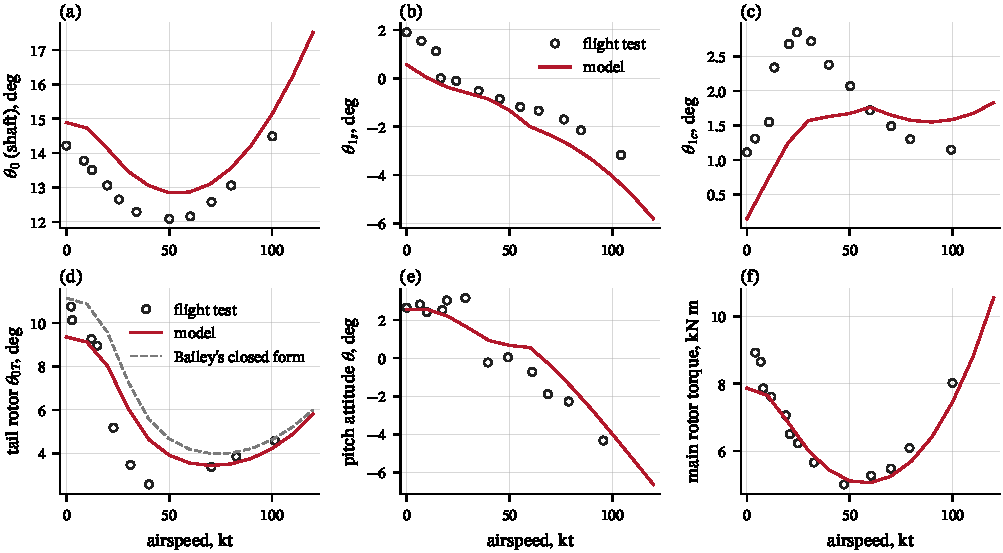
\includegraphics[width=\textwidth]{trim_dlr.pdf}
\caption{Level-flight trim against the DLR Bo 105-S123 as published by Padfield~\cite{pad}: 2200\,kg, sea level. Blade pitch harmonics in Helisim's
convention ($\theta_{1s}<0$ forward, $\theta_{1c}>0$ left), collective at the shaft; main rotor torque.}\label{fig:trimdlr}
\end{figure*}
\begin{figure*}[t]
\centering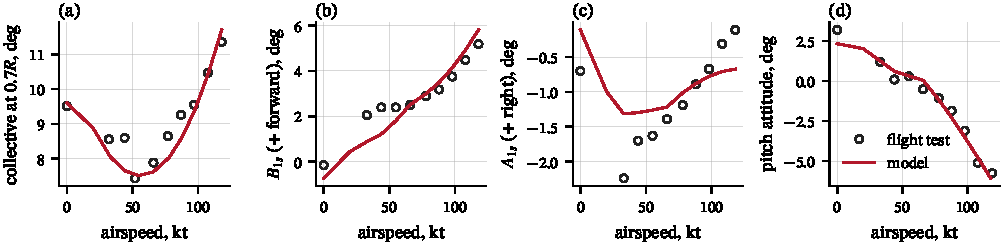
\includegraphics[width=\textwidth]{trim_mbb.pdf}
\caption{Level-flight trim against MBB's V-4 flight 108 as plotted in TR-75-50 fig.~16: 4500\,lb, 5000\,ft density altitude, CG 3.1\,in forward.}\label{fig:trimmbb}
\end{figure*}
\begin{table}[t]
\centering\small
\caption{Level-flight trim, model minus DLR test (deg); torque as model/test $-1$.}\label{tab:trimdlr}
\Tab{trim_dlr}
\end{table}
\begin{table}[t]
\centering\small
\caption{Level-flight trim, model minus MBB's test (deg), and the model's total power.}\label{tab:trimmbb}
\Tab{trim_mbb}
\end{table}

Against MBB's flight test (Fig.~\ref{fig:trimmbb}, Table~\ref{tab:trimmbb}) the model's collective at 0.7\,$R$ is within \NMcoll$^\circ$ at every speed,
its longitudinal cyclic within \NMlon$^\circ$ (\NMlonHi$^\circ$ from 55\,kt up), its lateral cyclic within \NMlat$^\circ$ and its pitch attitude within
\NMpitch$^\circ$. The power reaches its minimum of \NMpowMin\,hp near \NMpowMinV\,kt. The largest differences are in the transition, 33 to 44\,kt, where
the test needs about 1$^\circ$ more collective and 1.2$^\circ$ more forward cyclic than the model.

Against the DLR S123 (Fig.~\ref{fig:trimdlr}, Table~\ref{tab:trimdlr}) the model needs \NDthzMin--\NDthzMax$^\circ$ more collective than the test throughout,
and \NDlonMin--\NDlonMax$^\circ$ more forward cyclic, \NDlonMaxHi$^\circ$ at most from 60\,kt up. The lateral cyclic is within \NDlatMin{} to $+$\NDlatMax$^\circ$,
the largest differences at 10--30\,kt, where the test's lateral cyclic peaks with the onset of translational lift. The main rotor torque is within
\NDtqLow\,\% up to 60\,kt and falls to \NDtqMin\,\% of the test's at 90\,kt; at the lowest test speed, 4\,kt, the test reads \NDhoverTqTest\,kN\,m
and the model's hover \NDhoverTq. The tail rotor pitch (Fig.~\ref{fig:trimdlr}d) is \NTrBeHover$^\circ$ from the test's in the hover, \NTrBeTransMin--\NTrBeTransMax$^\circ$ above it from 20
to 40\,kt and within \NTrBeHi$^\circ$ from 60\,kt up. Bailey's closed form, which the model used before, is within \NTrBaHover$^\circ$ in the hover but
\NTrBaTransMin--\NTrBaTransMax$^\circ$ above the test through the transition and within \NTrBaHi$^\circ$ from 60\,kt up: the blade elements make more thrust
per degree and less of the hover's pitch, and follow the test's fall through the transition more closely. Both need \NTrBeHoverPow\,hp or so in
the hover. In the test the tail rotor's pitch drops by 4$^\circ$ between 12 and 23\,kt, which points to the fin and the tail rotor leaving the main
rotor's wake earlier than the ring wake has it. The fin blockage is small, as the fin stands in the pusher's inflow rather than its wake:
\NFinHoverPct\,\% of the tail rotor's thrust in the hover, \NFinPeakPct\,\% at \NFinPeakV\,kt, where the inflow's sidewash on the fin is
largest against the airspeed, and \NFinHiPct\,\% or less from 60\,kt up. It raises the pitch by \NFinDthHover$^\circ$ in the hover and
\NFinDthMax$^\circ$ at most, so it explains neither difference. The pitch attitude is within \NDpitchMax$^\circ$. The two
tests together suggest a model that is right in shape and slightly heavy in collective for the DLR aircraft, whose exact atmosphere is not published.
The model trims with \NDrollMax{} to \NDrollMin$^\circ$ of roll, left side down; no test value is published.

\subsection{The isolated rotor in hover}\label{sec:hover}
\begin{figure*}[t]
\centering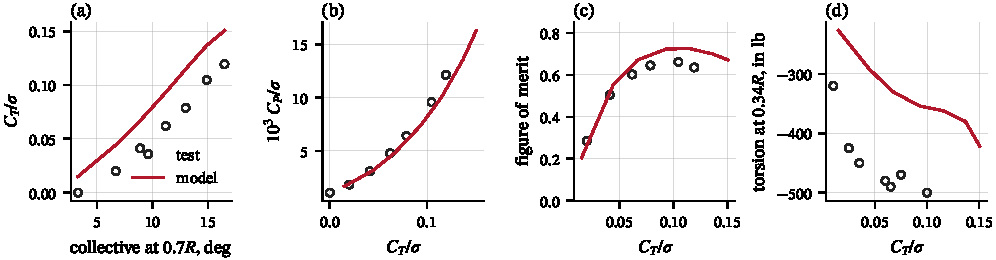
\includegraphics[width=\textwidth]{hover.pdf}
\caption{The isolated rotor in hover at 425\,rpm against NASA's full-scale test (TM-85892; torsion TM-103867): (a) thrust against collective at 0.7\,$R$,
(b) power against thrust, (c) figure of merit, (d) steady blade torsion moment at 0.34\,$R$.}\label{fig:hover}
\end{figure*}
\begin{table}[t]
\centering\small
\caption{The isolated rotor in hover: thrust at the test's collectives; power and figure of merit at the test's thrust.}\label{tab:hover}
\Tab{hover}
\end{table}

Here the model departs most clearly from a test (Fig.~\ref{fig:hover}, Table~\ref{tab:hover}). At the same collective it makes more thrust: the curves
are offset by \NHthMin--\NHthMax$^\circ$ of collective at equal $C_T/\sigma$, with nearly the same slope. At the test's thrust it needs \NHcpMin--\NHcpMax\,\% less
power, and its figure of merit peaks at \NHfmMod{} against the test's \NHfmTest. The steady torsion moment at 0.34\,$R$ has the test's trend but
\NHtorsMod{} against \NHtorsTest\,in\,lb at $C_T/\sigma=0.07$. In the flight trims the same rotor needs \emph{more} collective than the DLR aircraft
(above), so a collective offset in the model's rigging would not explain both. Possible causes, none verified: the tunnel test section in which
the rotor hovered recirculates part of the wake, which raises the inflow and the power at a given thrust; the test's collective was measured at
the blade's root, inboard of the control system's and the blade's elastic twist under the torsion moment, which the model's quasi-static torsion
mode represents with a lower moment; and the model's section drag is that of the smooth C-81 tables, without the increment for a tripped boundary
layer used for the UH-60. The tunnel's recirculation, if it is the cause, would put the model closer to free-air hover than the test.

\subsection{Blade dynamics}\label{sec:blades}
\begin{figure}[t]
\centering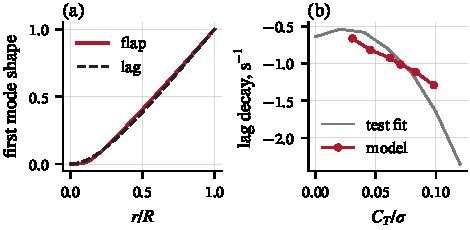
\includegraphics[width=\columnwidth]{blades.pdf}
\caption{(a) The first flap and lag modes. (b) Decay of the regressing lag mode in hover, 425\,rpm, against the curve fit through the full-scale rotor's
measurements (TM-85892 fig.~6).}\label{fig:blades}
\end{figure}
\begin{table}[t]
\centering\small
\caption{Blade frequencies per revolution at 425\,rpm: the beam model of TR-75-50's table 4 (torsion stiffness scaled), the model (lag stiffness tuned),
Boeing's Y-71 results and NASA's comprehensive analysis tuned to MBB's measurements.}\label{tab:blades}
\Tab{blades}
\end{table}
\begin{table}[t]
\centering\small
\caption{Lag damping in hover: decay coefficient of one blade's lag after a kick, and the full-scale rotor's (curve fit, TM-85892 fig.~6).}\label{tab:lag}
\Tab{lag}
\end{table}

The first flap, lag and torsion frequencies (Table~\ref{tab:blades}) are \NBflapMod, \NBlagMod{} and \NBtorsMod{} per revolution, against 1.12, 0.66 and 3.79
from NASA's analysis; the higher modes of the beam model agree with Boeing's to within 2\,\%, which checks the transcription of the structural data. The
lag damping (Fig.~\ref{fig:blades}b, Table~\ref{tab:lag}) is fitted at one point, $C_T/\sigma\approx0.07$, with a structural damping ratio of 1.7\,\%
(with 1\,\% the decay there was $-$0.77\,s$^{-1}$ against $-$0.97); the rest follows from the blades' aerodynamics. The model's decay grows with thrust as the
test's does, but less steeply: \NLagModLo{} against \NLagTestLo\,s$^{-1}$ at $C_T/\sigma=\NLagCtLo$ and \NLagModHi{} against \NLagTestHi{} at
\NLagCtHi. The fitted lag frequency is \NLagNu{} per revolution, on the 0.66 of the measurements.

\subsection{Derivatives and modes at 80\,kt}\label{sec:derivs}
\begin{table*}[t]
\centering\small
\caption{Derivatives at 80\,kt, 3000\,ft, 2200\,kg: the model, the DLR's identification, and the range of the six identifications of AGARD AR-280
(AFDD, CERT, DLR, Glasgow, NAE, NLR). Body axes at the CG, SI units, controls in \% of travel; $\uparrow\downarrow$: above or below the range.}\label{tab:derivs}
\Tab{derivs}
\end{table*}
\begin{table}[t]
\centering\small
\caption{Modes at 80\,kt: oscillatory [damping ratio, natural frequency in rad/s], aperiodic $1/T$ (s$^{-1}$, stable $>0$).}\label{tab:modes}
\Tab{modes}
\end{table}

Of the \NDerN{} derivatives that at least four of the six identifications include, \NDerIn{} of the model's lie within their range (Table~\ref{tab:derivs};
the model's trim at 80\,kt is \NDtheta$^\circ$ of pitch and \NDphi$^\circ$ of roll). Within it are the speed and heave derivatives $X_u$, $Z_u$ and
$Z_{\delta_c}$, the angle-of-attack stability $M_w$, the dihedral $L_v$ and the yaw damping $N_r$. The cyclic control powers lie above the range,
$M_{\delta_e}$ = \NdMlon{} against \NdMlonLo{} to \NdMlonHi{} and $L_{\delta_a}$ = \NdLlat{} against \NdLlatLo{} to \NdLlatHi, and the damping derivatives
further still: $M_q$ = \NdMq{} against \NdMqLo{} to \NdMqHi, $L_p$ = \NdLp{} against \NdLpLo{} to \NdLpHi. Their ratios, the steady rate per \% of cyclic,
are close to the DLR's: \NSsRoll{} against \NSsRollDlr\,rad/s per 100\,\% in roll and \NSsPitch{} against \NSsPitchDlr{} in pitch. A quasi-steady derivative
lets the rotor settle at each perturbation, which a 6-degree-of-freedom identification of an aircraft whose rotor lags the body cannot; the
identifications themselves differ by a factor of four in $L_p$. The directional stability $N_v$ = \NdNv{} is above the range (\NdNvLo{} to \NdNvHi). The
clearest disagreements are in the couplings: the roll due to longitudinal cyclic $L_{\delta_e}$
(\NdLlon{} against \NdLlonLo{} to \NdLlonHi), the roll due to collective $L_{\delta_c}$ (\NdLcol{} against \NdLcolLo{} to \NdLcolHi), the yaw due to roll rate $N_p$
(\NdNp{} against \NdNpLo{} to \NdNpHi) and the pitch due to collective, $M_{\delta_c}$ = \NdMcol{} (\NdMcolLo{} to \NdMcolHi). The C-81 analysis had the same
difficulty with the off-axis response~\cite{tr}. The modes (Table~\ref{tab:modes}) follow: the Dutch roll [\NMdrZeta, \NMdrW] has its damping within the identified
0.13--0.22 and its frequency \NMdrPct\,\% above the highest of 2.17--2.60; the phugoid [\NMphZeta, \NMphW] is unstable, as identified ($-$0.07 to $-$0.36); roll and short-period pitch combine into a
critically damped pair at \NMrpW\,rad/s, where the identifications find roll subsidences of 2.4--8.5\,s$^{-1}$ and pitch roots of 1.4--6.0.

\subsection{Roll frequency response}\label{sec:freq}
\begin{figure}[t]
\centering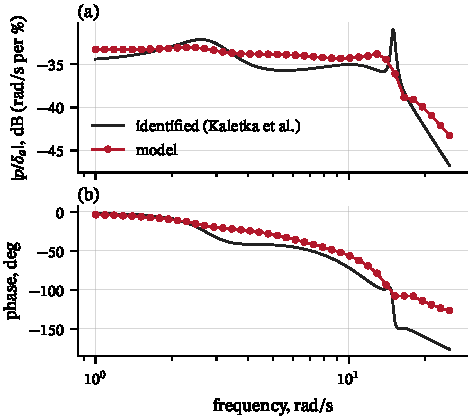
\includegraphics[width=\columnwidth]{freq.pdf}
\caption{Roll rate per \% lateral cyclic at 80\,kt: the model's frequency response from a lateral cyclic sweep, and the transfer function the DLR and the
AFDD identified from the flight frequency response (Kaletka et al.~\cite{kal}, with the lag/air resonance and the body roll/regressing flap mode).}\label{fig:freq}
\end{figure}
The frequency response (Fig.~\ref{fig:freq}) is the test that sees the rotor's dynamics directly. From 1 to 12\,rad/s the model's magnitude is within
\NFmagRms\,dB (rms, \NFmagMax{} at most) of the identified transfer function and its phase within \NFphRms$^\circ$ (rms); the model has a little less phase lag
between 3 and 12\,rad/s. The lag/air resonance appears at the identified frequency near 15\,rad/s with a similar notch and peak. Above it the model's phase lags
the identified by about \NFphHi$^\circ$ less; the identified function includes a 17\,ms time delay, which accounts for 15--25$^\circ$ there.

\subsection{Verification doublets}\label{sec:doublets}
\begin{figure*}[t]
\centering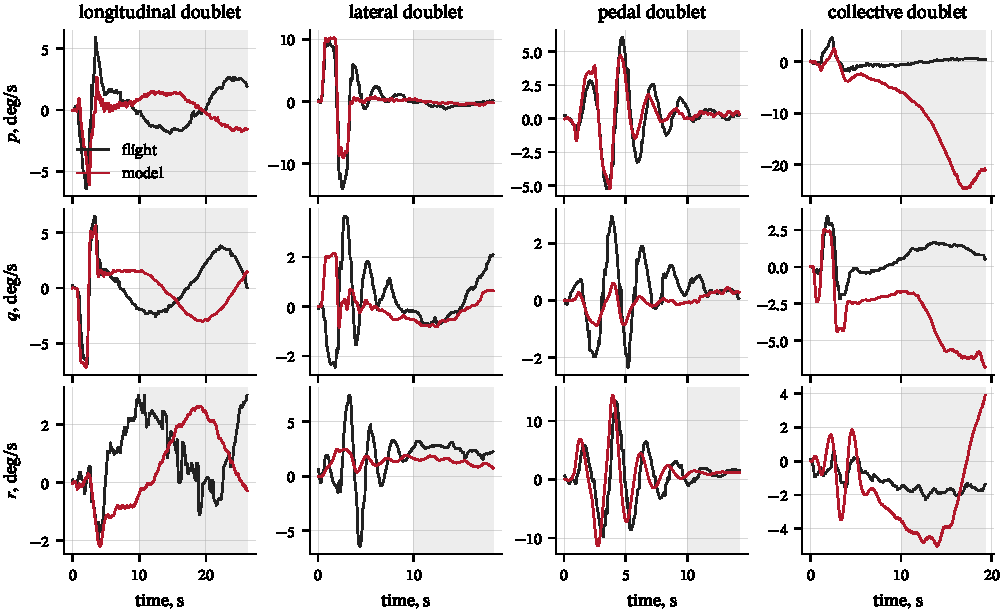
\includegraphics[width=\textwidth]{doublets.pdf}
\caption{Rate responses to the AGARD verification doublets at 80\,kt (AR-280 figs.~6.2.17 and 6.2.20): flight record and model, as increments from the
run's quiet window, with the recorded increments of all four controls applied to the model. Shaded: after the 10\,s used for the error.}\label{fig:doublets}
\end{figure*}
\begin{table}[t]
\centering\small
\caption{Verification doublets: rms error of the rate increments (rad/s) over the first 10\,s; bold: on axis.}\label{tab:doublets}
\Tab{doublets}
\end{table}
Over the first ten seconds (Fig.~\ref{fig:doublets}, Table~\ref{tab:doublets}) the on-axis rms error is \NDbOnDeg\,deg/s on average and \NDbAll\,deg/s over all
twelve traces. The pitch response to the longitudinal doublet peaks at \NDbLonPk\,deg/s against \NDbLonPkT, and the pedal doublet's yaw rate at
\NDbPedPk\,deg/s against \NDbPedPkT, its oscillation, the Dutch roll, in phase with the record. The lateral doublet's roll response is close in its first
second and then rings for longer than the aircraft's. The off-axis responses carry the couplings of Section~\ref{sec:derivs}: the pitch rate after the lateral
doublet is about half the record's, and the roll rate after the collective doublet has the wrong sign. After about ten seconds the model drifts away from the
aircraft in the longitudinal and collective runs, a pitch and roll divergence that the record does not show although the model receives the pilot's
recorded inputs; it is the long-term response of an unaugmented aircraft whose phugoid and speed stability differ slightly from the real one's.

\subsection{Rotor speed and engine response}\label{sec:engine}
\begin{figure*}[t]
\centering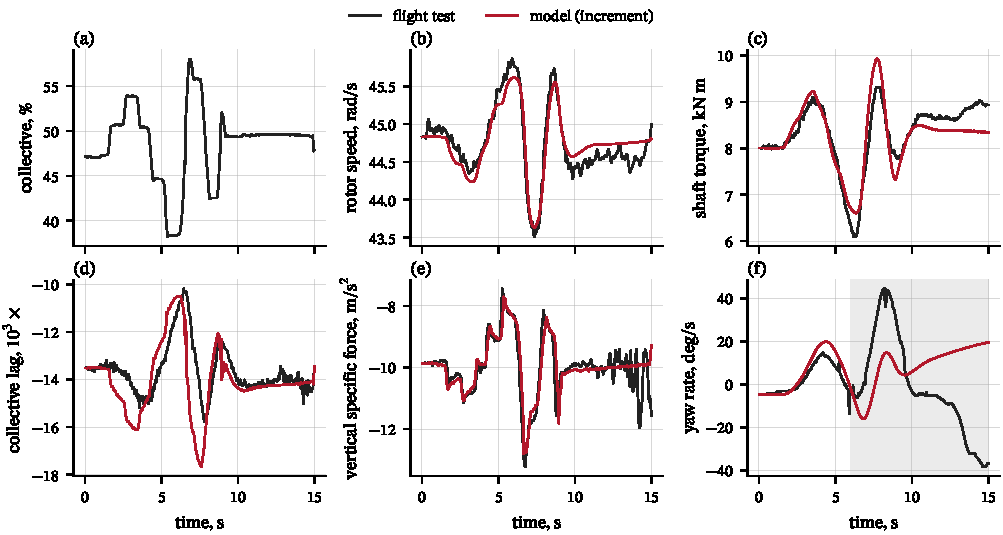
\includegraphics[width=\textwidth]{engine.pdf}
\caption{Collective 3-2-1-1 in hover against the DLR's flight test (Hamers and von Gr\"unhagen~\cite{hg}, fig.~6): (a) collective, (b) rotor speed, (c) shaft torque,
(d) collective lag (model: mean lag deflection at the tip over $R$), (e) vertical specific force, (f) yaw rate (the pilot's corrections after 6\,s, shaded, are not
known). Model as increments on the test's initial value.}\label{fig:engine}
\end{figure*}
\begin{table}[t]
\centering\small
\caption{Collective 3-2-1-1 in hover: lowest and highest increments in 15\,s (yaw rate: 6\,s) and the rms error.}\label{tab:engine}
\Tab{engine}
\end{table}
The governor's gain, lag and collective feed forward were fitted to this record, so it checks the structure rather than predicts (Fig.~\ref{fig:engine},
Table~\ref{tab:engine}). The rotor speed droops by \NEnrMinM\,rad/s against \NEnrMinT{} and overshoots by \NEnrMaxM{} against \NEnrMaxT, an rms error of
\NEnrRms\,rad/s (\NEnrPct\,\% of the rotor speed). The shaft torque's swing is a little larger than the test's on the way up (\NEtqMaxM{} against \NEtqMaxT\,kN\,m) and
smaller on the way down; the vertical specific force follows within \NEazRms\,m/s$^2$ rms. The blades' collective lag, which the DLR measured and the model
computes from its lag modes, follows the record in phase and amplitude. The yaw rate is comparable only in the first seconds, before the pilot's pedal.

% =====================================================================================================================
\section{Corrections found during validation}\label{sec:review}
The changes that the comparisons forced are listed here because each removed a physical or numerical inconsistency rather than tuning a coefficient.
\begin{enumerate}
\item \emph{Simulation rate.} The model first ran at 240\,Hz. There, and at 480\,Hz, the regressing lag mode coupled with the body's roll was under-damped or
unstable at 80\,kt, through explicit couplings in the step; at 960\,Hz its damping no longer changes, and the frequency response shows the identified air
resonance. FlightGear runs the model at 960\,Hz.
\item \emph{Rotor speed and lag together.} With the rotor speed and the blades' lag integrated one after the other, the lag modes, which carry most of the
blades' inertia about the shaft, and the drive exchanged their accelerations a step late. They are solved together.
\item \emph{The blades' inertia counted once.} The flap modes carry the blades' flapping inertia about the shaft's in-plane axes (317 of the rigid blades'
324\,slug\,ft$^2$); it is taken out of the airframe's roll and pitch inertias, which JSBSim would otherwise count twice.
\item \emph{The hub's acceleration.} The hub is 4.5\,ft above the centre of gravity; the blades now feel its specific force, including the airframe's
angular acceleration at that arm, as the airframe feels their in-plane forces at the same arm.
\item \emph{A second-order step for the blade modes.} A first-order step turned the flapping's phase by several degrees at 240\,Hz, through the half-step lag of
the strong aerodynamic damping.
\item \emph{Governor at flat pitch.} The collective feed forward fitted about the hover, held down to flat pitch, left the governor an 11\,\% droop there; the
rotor overshot to 107.5\,\% after a start. Below 35\,\% collective it now runs linearly to the gas generator speed the rotor needs at flat pitch, as a
compensator cam would; the start peaks at about 101\,\%, and the hover and forward flight stay on the fitted slope.
\item \emph{The 3-D model's rotor.} The FlightGear model's rotor stands 0.24\,m further aft of its nose than the flight manual's three-view shows; the
airframe's stations (skids, end plates, eye point, contacts) are taken from the manual's station diagram, and the visual rotor stays on the 3-D model's
mast. The trims, derivatives and responses were rerun after the change and did not move.
\end{enumerate}

% =====================================================================================================================
\section{Assessment}\label{sec:assess}
\begin{table}[t]
\centering\small
\caption{Summary: \ok{} within the test's scatter, \pok{} partly, \nok{} not reproduced.}\label{tab:score}
\begin{tabularx}{\columnwidth}{@{}>{\raggedright\arraybackslash}Xc@{}}
\toprule
Trim controls and attitudes against MBB's V-4, hover to 118\,kt & \ok \\
Trim against the DLR S123: pitch attitude, torque to 60\,kt & \ok \\
Collective and cyclic against the DLR S123 (up to \NDthzMax$^\circ$ and \NDlonMax$^\circ$) & \pok \\
Tail rotor pitch: transition (\NTrBeTransMin--\NTrBeTransMax$^\circ$ high), hover (\NTrBeHover$^\circ$) & \pok \\
Main rotor torque at 80--100\,kt (DLR) & \pok \\
Isolated rotor: thrust per collective, power per thrust & \nok \\
Blade frequencies & \ok \\
Lag damping against thrust (fitted at one point) & \pok \\
On-axis derivatives, directional stability, Dutch roll & \ok \\
Damping derivatives $L_p$, $M_q$ & \pok \\
Cross-coupling derivatives & \nok \\
Roll frequency response, 1--15\,rad/s, air resonance & \ok \\
On-axis doublet responses, first seconds & \ok \\
Off-axis doublet responses; long-term drift & \pok \\
Rotor speed after a collective 3-2-1-1 (fitted) & \ok \\
\bottomrule
\end{tabularx}
\end{table}
Table~\ref{tab:score} summarises. The model reproduces what distinguishes the Bo 105, its blades' dynamics and the quick on-axis response of the hingeless rotor,
together with the trims of MBB's prototype. Its open items are the isolated rotor's thrust and power against NASA's hover test, which the flight trims do not
confirm and whose cause is open, the tail rotor's pitch through the transition, the cross-couplings, where the model shares the C-81 analysis's difficulty,
and the long-term response of the free aircraft. The tail rotor's blade elements have a stall and reversed flow, but no published test checks them at the tail rotor's
limits, in strong crosswinds or near its stall, and its section is C-81's equations rather than measured tables. Ground effect uses the UH-60's chart for want of the
Bo 105's.

% =====================================================================================================================
\section{Conclusions}\label{sec:concl}
\begin{itemize}
\item An elastic-blade model of the Bo 105's hingeless rotor, with individual blades, their first flap and lag bending modes and a quasi-static torsion mode, a
finite-state dynamic wake, the C-81 airframe and two 250-C20B engines, runs in plain JSBSim, generated from data. It is the flight model of the FlightGear Bo 105.
\item The blade frequencies from the published structural data, with the lag stiffness tuned to MBB's measured frequency, and the lag damping fitted at one
point, give the roll response at 80\,kt with the air resonance where the DLR identified it.
\item Against MBB's flight test the trims are within about a degree of every control from hover to 118\,kt; against the DLR's aircraft the collective is
\NDthzMin--\NDthzMax$^\circ$ high and the tail rotor's pitch falls later through the transition than in the test.
\item Against NASA's full-scale hover test the rotor makes more thrust per degree of collective and needs less power per unit thrust; the cause is open.
\item A blade-element teetering tail rotor with C-81's 0012 equations follows the DLR aircraft's tail rotor pitch through the transition
about a degree closer than Bailey's closed form, and is \NTrBeHover$^\circ$ from the test in the hover.
\item The air resonance sets the simulation rate: an explicit integration needs 960\,Hz for the coupled lag and body modes.
\item The cross-coupling derivatives at 80\,kt and the free aircraft's long-term drift are documented, not tuned away.
\end{itemize}

\begin{thebibliography}{99}\small
\bibitem{tr} Boeing Vertol Company, \emph{Validation of Rotorcraft Flight Simulation Program through Correlation with Flight Data for Soft-in-Plane Hingeless Rotors}, USAAMRDL TR 75-50, 1976.
\bibitem{pt} R.\,L.\ Peterson and W.\ Johnson, \emph{Aeroelastic Loads and Stability Investigation of a Full-Scale Hingeless Rotor}, NASA TM-103867, 1991.
\bibitem{pw} R.\,L.\ Peterson and W.\ Warmbrodt, \emph{Hover Test of a Full-Scale Hingeless Helicopter Rotor: Aeroelastic Stability, Performance, and Loads Data}, NASA TM-85892, 1984.
\bibitem{wp} W.\ Warmbrodt and R.\,L.\ Peterson, \emph{Hover Test of a Full-Scale Hingeless Rotor}, NASA TM-85990, 1984.
\bibitem{pm} R.\,L.\ Peterson, \emph{Full-Scale Hingeless Rotor Performance and Loads}, NASA TM-110356, 1995.
\bibitem{hf} R.\,K.\ Heffley et al., \emph{A Compilation and Analysis of Helicopter Handling Qualities Data, Volume One: Data Compilation}, NASA CR-3144, 1979.
\bibitem{ar} AGARD, \emph{Rotorcraft System Identification}, AGARD Advisory Report 280, 1991.
\bibitem{kal} J.\ Kaletka, M.\,B.\ Tischler, W.\ von Gr\"unhagen and J.\,W.\ Fletcher, \emph{Time and Frequency-Domain Identification and Verification of BO 105 Dynamic Models}, 15th European Rotorcraft Forum, paper 66, 1989.
\bibitem{hg} M.\ Hamers and W.\ von Gr\"unhagen, \emph{Dynamic Engine Model Integrated in Helicopter Simulation}, 23rd European Rotorcraft Forum, paper 91, 1997.
\bibitem{pad} G.\,D.\ Padfield, \emph{Helicopter Flight Dynamics}, 3rd ed., Wiley, 2018.
\bibitem{metu} Middle East Technical University, M.Sc.\ thesis on forward flight trim and longitudinal stability codes (Peters--He finite-state wake; Padfield's Bo 105 data).
\bibitem{ea} European Union Aviation Safety Agency, \emph{Type-Certificate Data Sheet EASA.R.011, BO105}, issue 3, 2017.
\bibitem{fm} Eurocopter, \emph{BO 105 CB-5/CBS-5 Flight Manual}.
\bibitem{heyson} H.\,H.\ Heyson, \emph{Ground Effect for Lifting Rotors in Forward Flight}, NASA TN D-234, 1960.
\bibitem{hk} H.\,H.\ Heyson and S.\ Katzoff, \emph{Induced Velocities Near a Lifting Rotor with Nonuniform Disk Loading}, NACA Report 1319, 1957.
\bibitem{jsbsim} JSBSim Development Team, \emph{JSBSim: an open-source flight dynamics model}, version 1.3.3.
\end{thebibliography}
\end{document}
